\chapter{Metoda rozwiązania problemu}\label{algo}
\section{Opis}
Rozwiązanie problemu usuwania obiektów dynamicznych z sekwencji obrazów wymagało zastosowania kilku etapów. Poniżej przedstawiono sposób rozwiązania każdego z nich.

\subsection{Dopasowywanie obrazów}
W pierwszym etapie należało dopasować do siebie poszczególne obrazy tak, aby piksele na kolejnych ujęciach odpowiadały sobie. Aby tego dokonać należy wybrać arbitralnie obraz referencyjny do którego będą dopasowywane pozostałe ujęcia (w tym przypadku środkowy obraz z sekwencji). Następnie każdy z obrazów zostaje poddany transformacji perspektywicznej do współrzędnych obrazu referencyjnego. Poniżej przedstawiono graficzną reprezentację tego zagadnienia.

\begin{figure}[H]
	\centering
		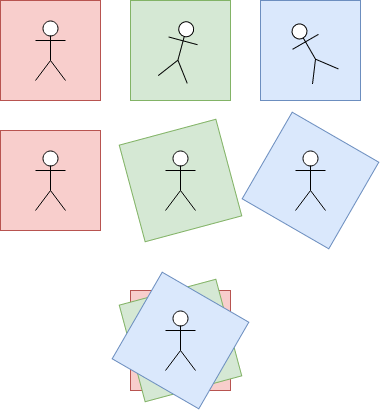
\includegraphics[width=0.5\linewidth]{img/matching.png}
	\caption[Dopasowanie obrazów.]{Dopasowanie obrazów. Czerwonym kolorem zaznaczono obraz referencyjny.}
	\label{fig:binary}
\end{figure}

W celu uzyskania dopasowania zastosowano algorytm detekcji i deskrypcji punktów kluczowych (AKAZE) na obrazach. Następnie zastosowano Algorytm przeglądu zupełnego (BFMatcher) do znalezienia najbliższych punktów odpowiadających sobie na dwóch obrazach. Uzyskany w ten sposób zestaw par punktów kluczowych zostaje użyty do znalezienia transformacji perspektywicznej. Do tego celu użyto metodę RANSAC, która w sposób losowy wybiera zestaw punktów i oblicza macierz transformacji. Wielokrotne powtórzenie tego procesu pozwala na znalezienie wystarczająco dokładnej macierzy transformacji.
\subsection{Usuwanie obiektów}

Zaproponowana metoda usuwania obiektów dynamicznych opiera się na analizie serii pikseli pochodzących z kolejnych dopasowanych względem siebie klatek. W pierwszym kroku pobierany jest wektor pikseli (z konkretnej pozycji na obrazie) reprezentujących ich wartości na kolejnych klatkach obrazu. Następnie tak utworzony zbiór punktów poddawany jest kolejnym funkcją, tak aby uzyskać piksel który możliwie najlepiej odwzorowuje tło. W tym celu stosowane są sekwencyjnie różne funkcje statystyczne, które redukują ilość pikseli w wektorze, aż do pozostawienia pojedynczego piksela. Poniżej przedstawiono graficzną reprezentację tego procesu.

\begin{figure}[H]
	\centering
		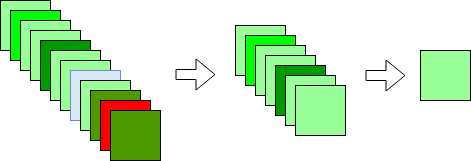
\includegraphics[width=0.75\linewidth]{img/process.png}
	\caption[Redukcja ilości pikseli.]{Proces redukowania ilości pikseli.}
	\label{fig:binary}
\end{figure}

Dokonywanie redukcji ilości pikseli kandydujących realizowane jest przez zastosowanie pewnych funkcji. Każda z nich operuje na pewnym fragmencie oryginalnego wektora i eliminuje z niego część lub wszystkie piksele. Poniżej znajduje się ich opis:
\begin{itemize}
\item median - wartość środkowa 
\item mean - piksel o najbliżej wartości do średniej
\item outliers - usuwanie pikseli o wartościach większych niż odchylenie standardowe pomnożone przez dany współczynnik
\item remove-unstable - usuwanie serii pikseli, gdy ich odchylenie standardowe ich wartości przekroczy zadany próg
\item most-stable - znalezienie serii pikseli o wartościach z najniższym odchyleniu standardowym
\end{itemize}

Sposób obliczania wartości danego piksela jest wykonywany różnymi sposobami:
\begin{itemize}
\item channel - wybór odpowiedniego kanału dla piksela
\item length - długość wektora wyznaczonego przez piksel w danej metryce
\item vector - suma długości wektorów różnic pewnego piksela od pozostałych w danej metryce
\end{itemize}

Powyżej opisane funkcje mogą być szeregowane względem siebie w dowolny sposób z dowolnymi parametrami.
\newpage
\section{Algorytm}

\begin{enumerate}
\item Wybór obrazu referencyjnego $I_r$
\item Dla każdego obrazu $I_k$ należącego do sekwencji:
\begin{enumerate}
\item Znalezienie punktów kluczowych na obu obrazach $I_k$, $I_r$
\item Parowanie punktów kluczowych na dwóch obrazach
\item Obliczenie macierzy transformacji perspektywicznej
\item Przekształcenie obrazu $I_k$ do współrzędnych obrazu $I_r$
\end{enumerate}
\item Dla każdej pozycji w obrazie wyjściowym znaleźć odpowiadającą serię pikseli z pozostałych obrazów
\begin{enumerate}
\item Dla każdej funkcji $f$ w potoku
\begin{enumerate}
\item Redukcja serii pikseli w wyniku zastosowania funkcji $f$
\end{enumerate}
\item Skopiowanie wartości pozostałego piksela w odpowiednie miejsce obrazu wyjściowego.
\end{enumerate}
\end{enumerate}
